% ============================================================================
% AOGS study — illustrated plain-language explainer (PDF companion to
% AOGS_STUDY_EXPLAINER.md). Embeds the pipeline flowchart, the K_d bowl,
% the four poster data figures, and three inline concept diagrams.
% Numbers via poster_numbers.tex (generated, never hand-typed).
% Build:  /Library/TeX/texbin/pdflatex aogs_study_explainer.tex   (x2)
% ============================================================================
\documentclass[11pt]{article}
\usepackage[a4paper, margin=20mm]{geometry}
\usepackage[T1]{fontenc}
\usepackage{newtxtext,newtxmath}
\usepackage{graphicx}
\usepackage{booktabs}
\usepackage{xcolor}
\usepackage{tikz}
\usepackage[font=small,labelfont=bf]{caption}
\usepackage{enumitem}
\usepackage{amsmath}
\usepackage{float}
\usetikzlibrary{positioning, arrows.meta, calc}
\newcommand{\horAfif}{14.0}
\newcommand{\lossAfif}{1.16}
\newcommand{\svfAfif}{0.985}
\newcommand{\kdstarAfif}{4.60}
\newcommand{\horAsev}{10.1}
\newcommand{\lossAsev}{0.18}
\newcommand{\svfAsev}{0.991}
\newcommand{\kdstarAsev}{7.08}
\newcommand{\rmsehayAfif}{2.03}
\newcommand{\rmsecpAfif}{1.74}
\newcommand{\bestzcpAfif}{5/30}
\newcommand{\bestrhocpAfif}{1500/1700/1700}
\newcommand{\rmsecKAfif}{0.90}
\newcommand{\bestzcKAfif}{10/30}
\newcommand{\bestrhocKAfif}{1500/1700/1800}
\newcommand{\rmsehayAsev}{0.54}
\newcommand{\rmsecpAsev}{0.39}
\newcommand{\bestzcpAsev}{5/30}
\newcommand{\bestrhocpAsev}{1500/1700/1700}
\newcommand{\rmsecKAsev}{0.36}
\newcommand{\bestzcKAsev}{5/30}
\newcommand{\bestrhocKAsev}{1300/1500/1900}
\newcommand{\rmsehomAfif}{2.31}
\newcommand{\rmsehomAsev}{3.76}
\newcommand{\xferatAsev}{1.64}
\newcommand{\xferatAfif}{1.73}
\newcommand{\svfdtirAfif}{1.15}
\newcommand{\svfdtallAfif}{1.30}
\newcommand{\svfdtirAsev}{0.65}
\newcommand{\svfdtallAsev}{0.74}
\newcommand{\shadowcoolAfif}{2.22}
\newcommand{\shadowcoolAsev}{0.48}
\newcommand{\stabcKAfif}{13}
\newcommand{\bootcicKAfif}{0.26--1.08}
\newcommand{\stabcKAsev}{36}
\newcommand{\bootcicKAsev}{0.25--0.43}
\newcommand{\driftmax}{35}
\newcommand{\closurewin}{0.70}


\definecolor{teal}{HTML}{2A6478}
\definecolor{coral}{HTML}{B85B3A}
\definecolor{forest}{HTML}{3D6E4A}
\definecolor{char}{HTML}{2A2520}
\definecolor{gridc}{HTML}{E8E5E0}
\definecolor{dim}{HTML}{8A857E}
\color{char}

\graphicspath{{../figures/poster/}{../figures/diagrams/}{../figures/explainers/}}

\tikzset{
  newbox/.style={draw=teal, fill=teal!9, rounded corners=2.5pt, line width=0.8pt,
                 align=center, inner sep=4pt, text=char, font=\small},
  greybox/.style={draw=dim, fill=gridc, rounded corners=2.5pt, line width=0.8pt,
                  align=center, inner sep=4pt, text=char, font=\small},
  warnbox/.style={draw=coral, fill=coral!11, rounded corners=2.5pt, line width=0.8pt,
                  align=center, inner sep=4pt, text=char, font=\small},
  arr/.style={-{Stealth[length=2.2mm]}, draw=dim, line width=0.8pt,
              rounded corners=2pt, line cap=round},
}
\setlist[itemize]{leftmargin=1.4em, itemsep=1pt, topsep=2pt}
\newcommand{\shead}[1]{\medskip\noindent{\color{teal}\large\bfseries #1}\par\nobreak\smallskip}

\begin{document}
\thispagestyle{empty}

\begin{center}
{\LARGE\bfseries Discrete-Layer Lunar Thermal Modeling}\\[2pt]
{\large\color{teal}\bfseries A plain-language explainer of the AOGS study}\\[4pt]
{\small Ram\'on III P.\ Gregorio \quad$\bullet$\quad Institute of Science Tokyo
 \,/\, Kasai Laboratory, NICT}\\[-2pt]
{\footnotesize\color{dim} companion to the poster; every number from the results
 archives}
\end{center}
\vspace{2pt}
{\color{teal}\rule{\linewidth}{0.9pt}}

% ── 1 ───────────────────────────────────────────────────────────────────────
\shead{1.\ \ What this study is, in one sentence}
It is an \textbf{extension of the JGR letter}. The letter retrieved one deep
regolith conductivity $K_d$ per Apollo borehole; this study asks what
\emph{layered density structure} best explains the same temperatures, and adds
\textbf{topographic shadowing} from the real terrain. Same certified physics
engine, two new ingredients, and the product is a validated
\emph{thermal profile} plus a thermally-retrieved density column.

\begin{figure}[h]\centering
  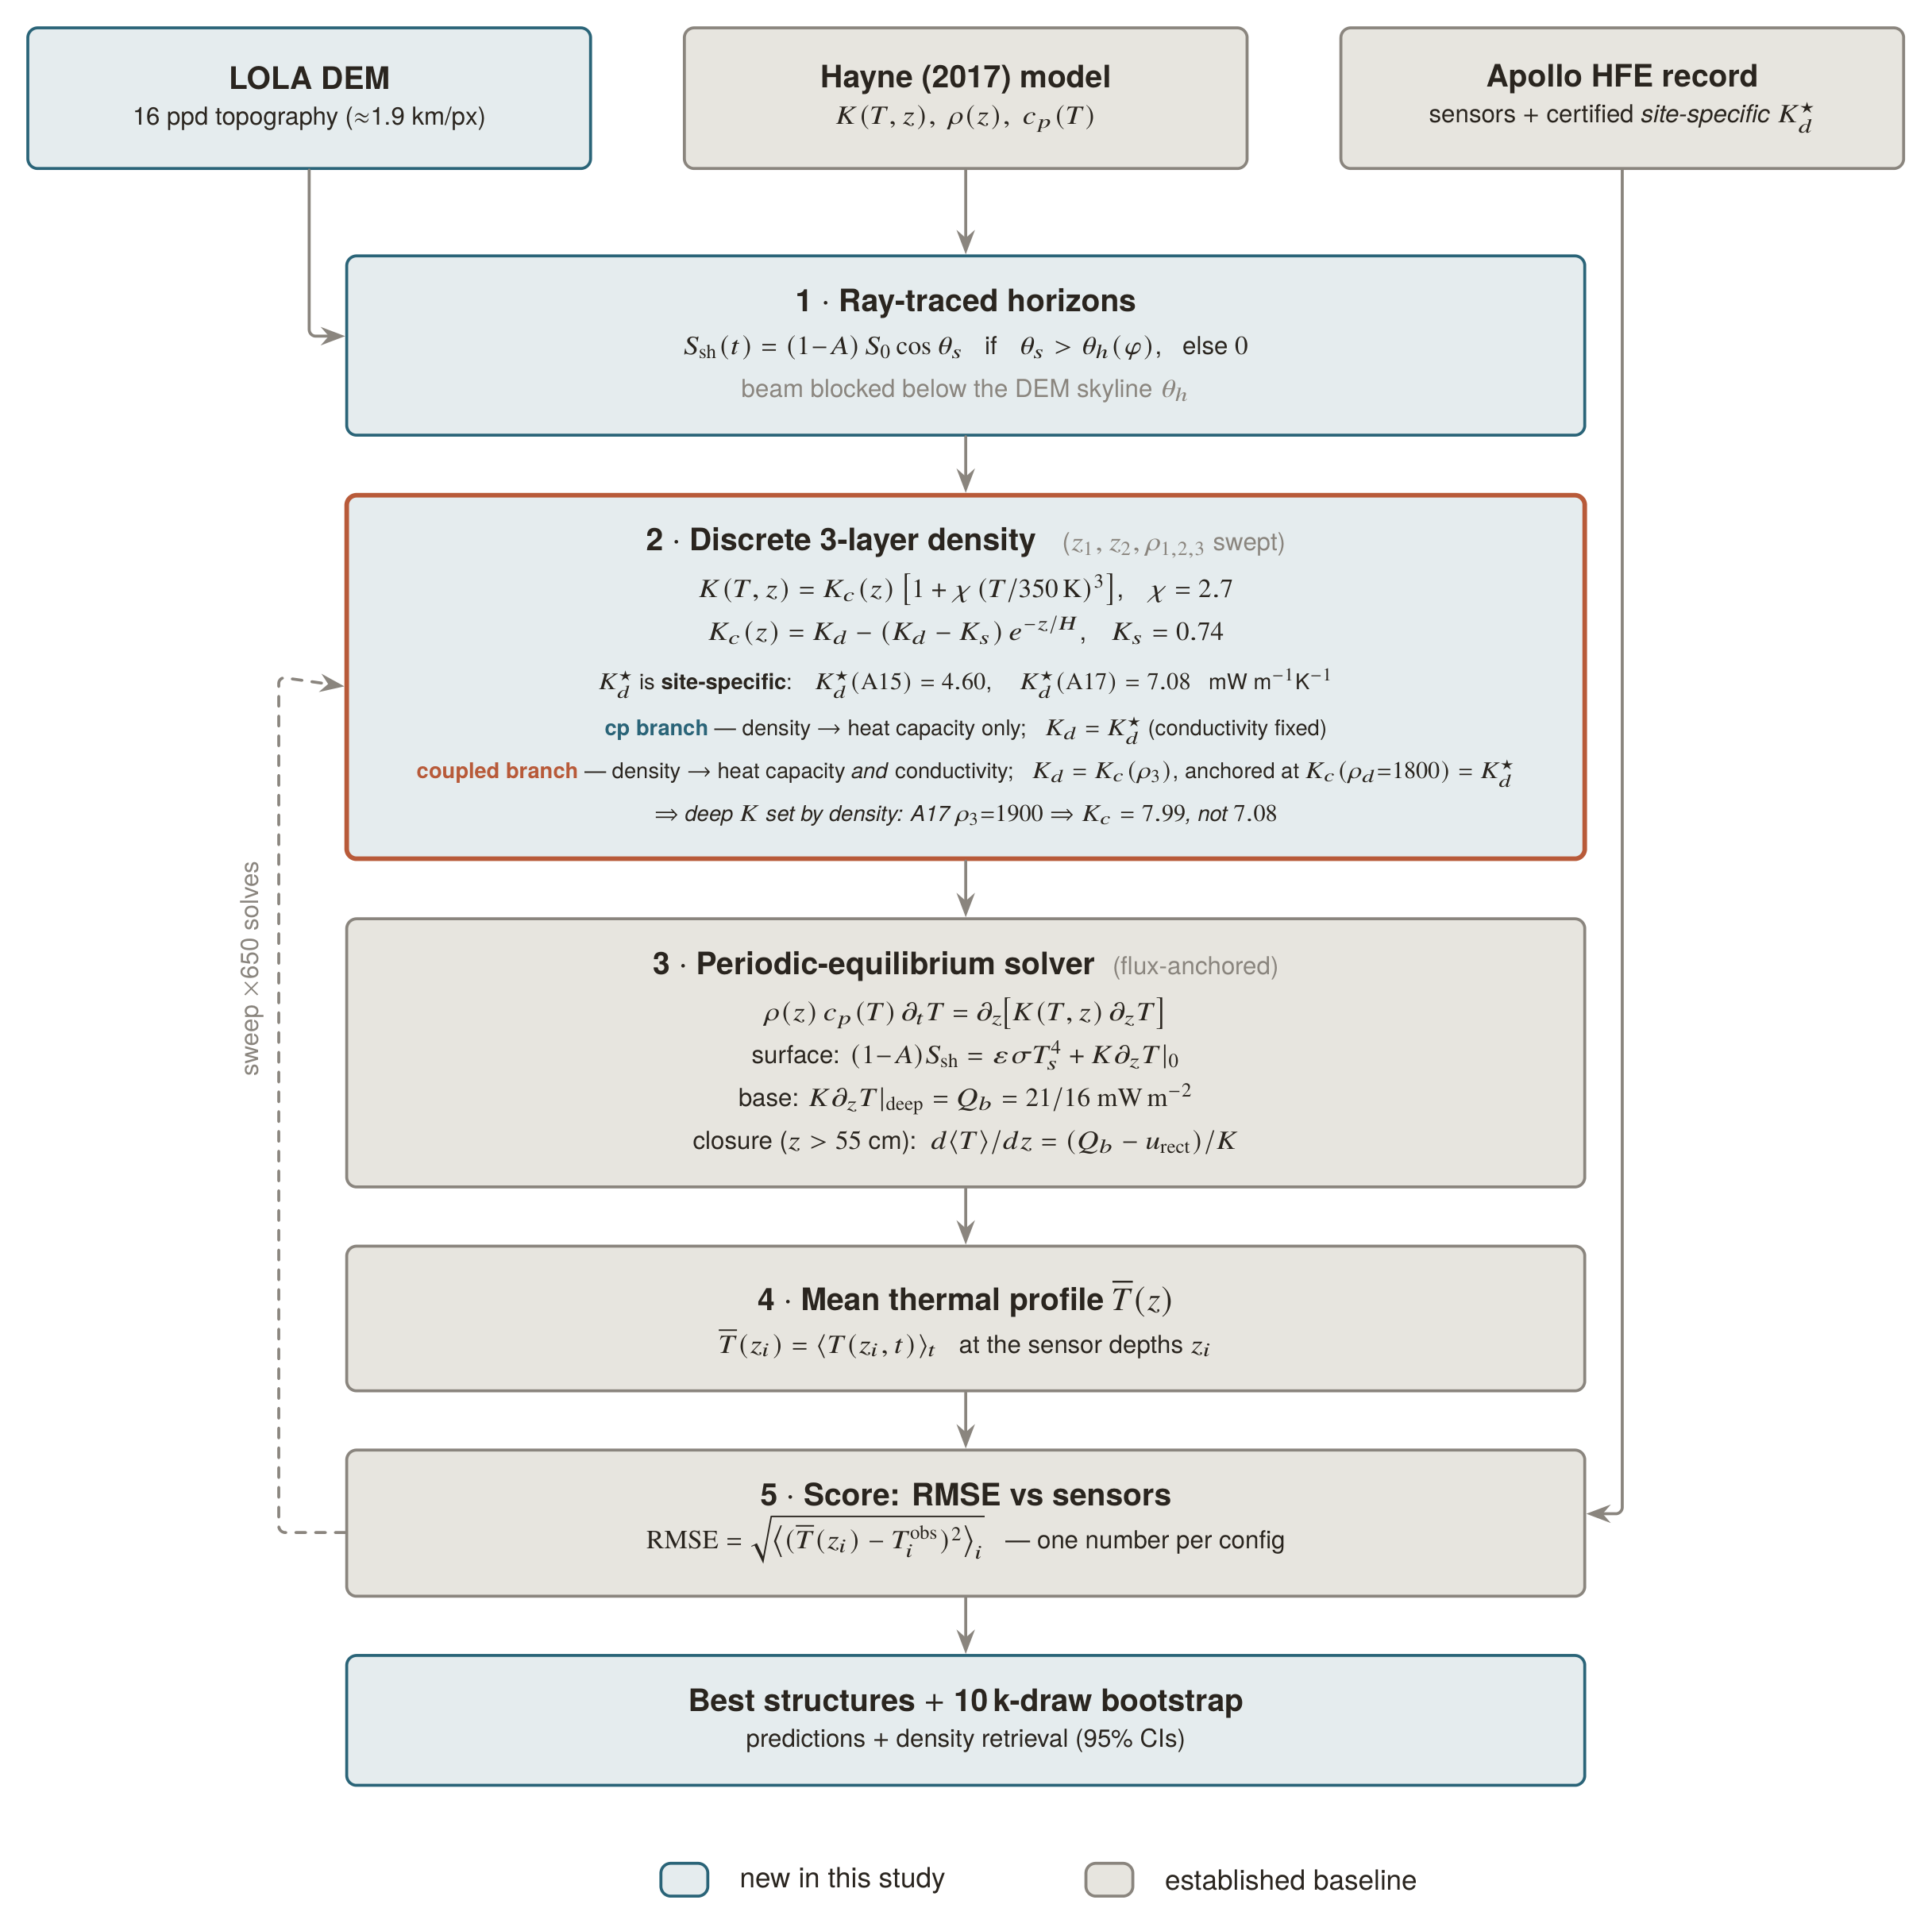
\includegraphics[width=0.62\linewidth]{aogs_pipeline_flowchart.pdf}
  \caption{The pipeline. Teal boxes are new in this study; grey boxes are
  inherited from the letter's certified solver. Three inputs feed a five-stage
  loop run over 650 layer configurations.}
\end{figure}

% ── 2 ───────────────────────────────────────────────────────────────────────
\shead{2.\ \ The engine we reuse (nothing new here)}
The same Hayne et al.\ (2017) physics as the letter. Heat moves in a 1-D column
by conduction, $\rho(z)\,c_p(T)\,\partial_t T=\partial_z[K\,\partial_z T]$, with
a two-part conductivity
\[
  K(T,z)=K_c(z)\,\bigl[1+\chi\,(T/350\,\mathrm{K})^3\bigr],
\]
grain-contact conduction \emph{plus} radiative transfer between grains. The
surface energy balance sets the top; a fixed geothermal flux $Q_b$ sets the
bottom. We solve for the \emph{repeating} lunar-day cycle and read off
$\overline{T}(z)$, the time-averaged temperature vs depth, at the Apollo sensor
depths.

% ── 3 ───────────────────────────────────────────────────────────────────────
\shead{3.\ \ The two things we add}
\begin{itemize}
  \item \textbf{Topographic shadowing.} Ray-tracing the LOLA DEM gives each
    borehole's skyline; the Sun below it is blocked. Apollo~15 loses
    \lossAfif\% of its sunlight (Apennine front), Apollo~17 \lossAsev\%
    (North Massif).
  \item \textbf{Discrete density layers.} Instead of one smooth Hayne density
    curve, a \textbf{3-layer staircase} --- loose surface, intermediate,
    compact deep --- with density rising with depth.
\end{itemize}

% ── 4 density model ──────────────────────────────────────────────────────────
\shead{4.\ \ What density profiles we test}
Three layers, each denser than the one above (regolith compacts with depth,
never the reverse). The boundaries and densities are swept over a grid.

\begin{figure}[h]\centering
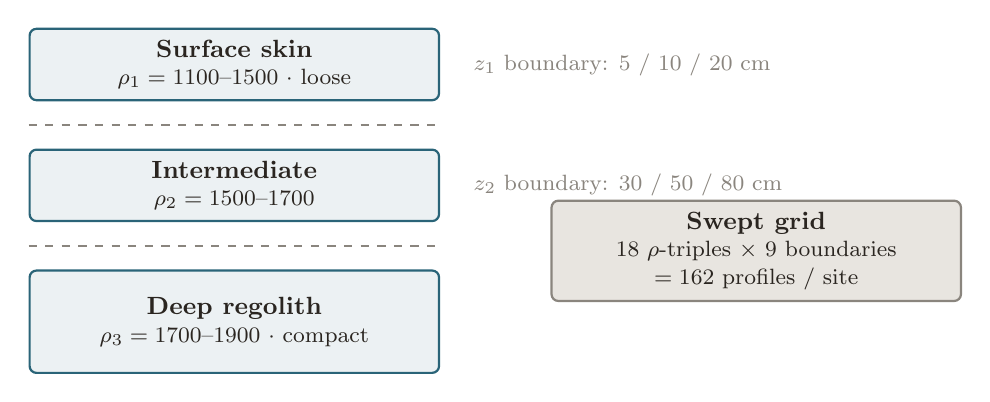
\begin{tikzpicture}[node distance=2mm]
  \node[newbox, minimum width=52mm, minimum height=9mm] (skin)
    {\textbf{Surface skin}\\[-1pt]{\footnotesize $\rho_1=1100\text{--}1500$ $\cdot$ loose}};
  \node[newbox, minimum width=52mm, minimum height=9mm, below=6mm of skin] (mid)
    {\textbf{Intermediate}\\[-1pt]{\footnotesize $\rho_2=1500\text{--}1700$}};
  \node[newbox, minimum width=52mm, minimum height=13mm, below=6mm of mid] (deep)
    {\textbf{Deep regolith}\\[-1pt]{\footnotesize $\rho_3=1700\text{--}1900$ $\cdot$ compact}};
  \node[right=3mm of skin.east, font=\footnotesize, text=dim, anchor=west]
    {$z_1$ boundary: 5 / 10 / 20 cm};
  \node[right=3mm of mid.east, font=\footnotesize, text=dim, anchor=west]
    {$z_2$ boundary: 30 / 50 / 80 cm};
  \node[greybox, right=14mm of deep.east, minimum width=52mm, anchor=west,
        yshift=9mm] (grid)
    {\textbf{Swept grid}\\[-1pt]{\footnotesize 18 $\rho$-triples $\times$ 9
     boundaries}\\[-1pt]{\footnotesize $=162$ profiles / site}};
  \draw[dim, dashed, line width=0.6pt] (skin.south west)++(0,-3mm)
        -- ($(skin.south east)+(0,-3mm)$);
  \draw[dim, dashed, line width=0.6pt] (mid.south west)++(0,-3mm)
        -- ($(mid.south east)+(0,-3mm)$);
\end{tikzpicture}
\caption{The 3-layer density model. Densities in kg\,m$^{-3}$; the monotone
rule $\rho_1\le\rho_2\le\rho_3$ leaves 162 profiles per site per branch. Two
branches: \textbf{cp} (density $\to$ heat capacity only) and \textbf{coupled}
(density $\to$ conductivity too, through the Hayne form's own $K_c(\rho)$).}
\end{figure}

\begin{figure}[h]\centering
  \includegraphics[width=0.60\linewidth]{poster_density.pdf}
  \caption{What the data prefer: the winning 3-layer staircases (green A15,
  coral A17) against Hayne's smooth continuous profile (dotted). Both want a
  \emph{denser-than-Hayne} surface and the compaction step \emph{high} in the
  column.}
\end{figure}

% ── 5 degeneracy ─────────────────────────────────────────────────────────────
\shead{5.\ \ The key subtlety: $K_d\leftrightarrow$ density degeneracy}
The deep temperature gradient is essentially $Q_b/K_\mathrm{deep}$.
\emph{Both} a higher $K_d$ \emph{and} a denser deep layer raise
$K_\mathrm{deep}$ --- they give the same gradient. So the sensors alone
\textbf{cannot separate them}.

\begin{figure}[h]\centering
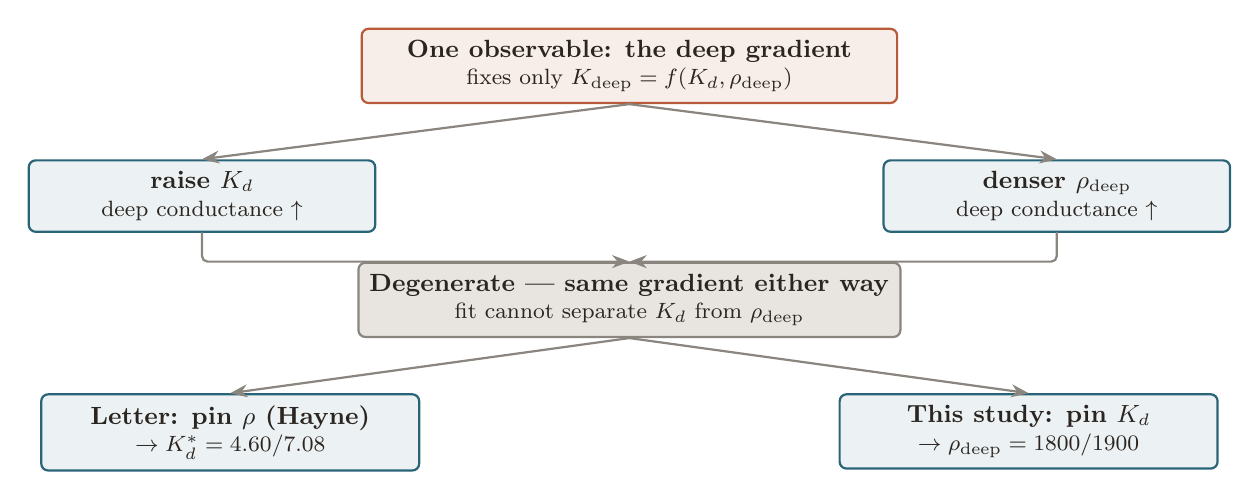
\begin{tikzpicture}
  \node[warnbox, minimum width=68mm] (obs)
    {\textbf{One observable: the deep gradient}\\[-1pt]
     {\footnotesize fixes only $K_\mathrm{deep}=f(K_d,\rho_\mathrm{deep})$}};
  \node[newbox, below left=7mm and -2mm of obs, minimum width=44mm] (ka)
    {\textbf{raise $K_d$}\\[-1pt]{\footnotesize deep conductance $\uparrow$}};
  \node[newbox, below right=7mm and -2mm of obs, minimum width=44mm] (kb)
    {\textbf{denser $\rho_\mathrm{deep}$}\\[-1pt]{\footnotesize deep conductance $\uparrow$}};
  \node[greybox, below=20mm of obs, minimum width=64mm] (deg)
    {\textbf{Degenerate --- same gradient either way}\\[-1pt]
     {\footnotesize fit cannot separate $K_d$ from $\rho_\mathrm{deep}$}};
  \node[newbox, below left=7mm and -8mm of deg, minimum width=48mm] (let)
    {\textbf{Letter: pin $\rho$ (Hayne)}\\[-1pt]{\footnotesize $\to K_d^{*}=\kdstarAfif/\kdstarAsev$}};
  \node[newbox, below right=7mm and -8mm of deg, minimum width=48mm] (stu)
    {\textbf{This study: pin $K_d$}\\[-1pt]{\footnotesize $\to \rho_\mathrm{deep}=1800/1900$}};
  \draw[arr] (obs.south) -- (ka.north);
  \draw[arr] (obs.south) -- (kb.north);
  \draw[arr] (ka.south) |- (deg.north);
  \draw[arr] (kb.south) |- (deg.north);
  \draw[arr] (deg.south) -- (let.north);
  \draw[arr] (deg.south) -- (stu.north);
\end{tikzpicture}
\caption{Why $K_d$ and deep density can't be pinned together. In the
\emph{coupled} branch the winner's effective deep conductivity is
$K_c(\rho_3)$, not $K_d^{*}$: A15's $\rho_3{=}1800$ gives 4.60 (unchanged);
A17's $\rho_3{=}1900$ gives 7.99 (shifted $+0.91$). ``$K_d^{*}{=}7.08$ and
$\rho_3{=}1900$'' are two descriptions of one deep-gradient requirement.}
\end{figure}

\begin{figure}[h]\centering
  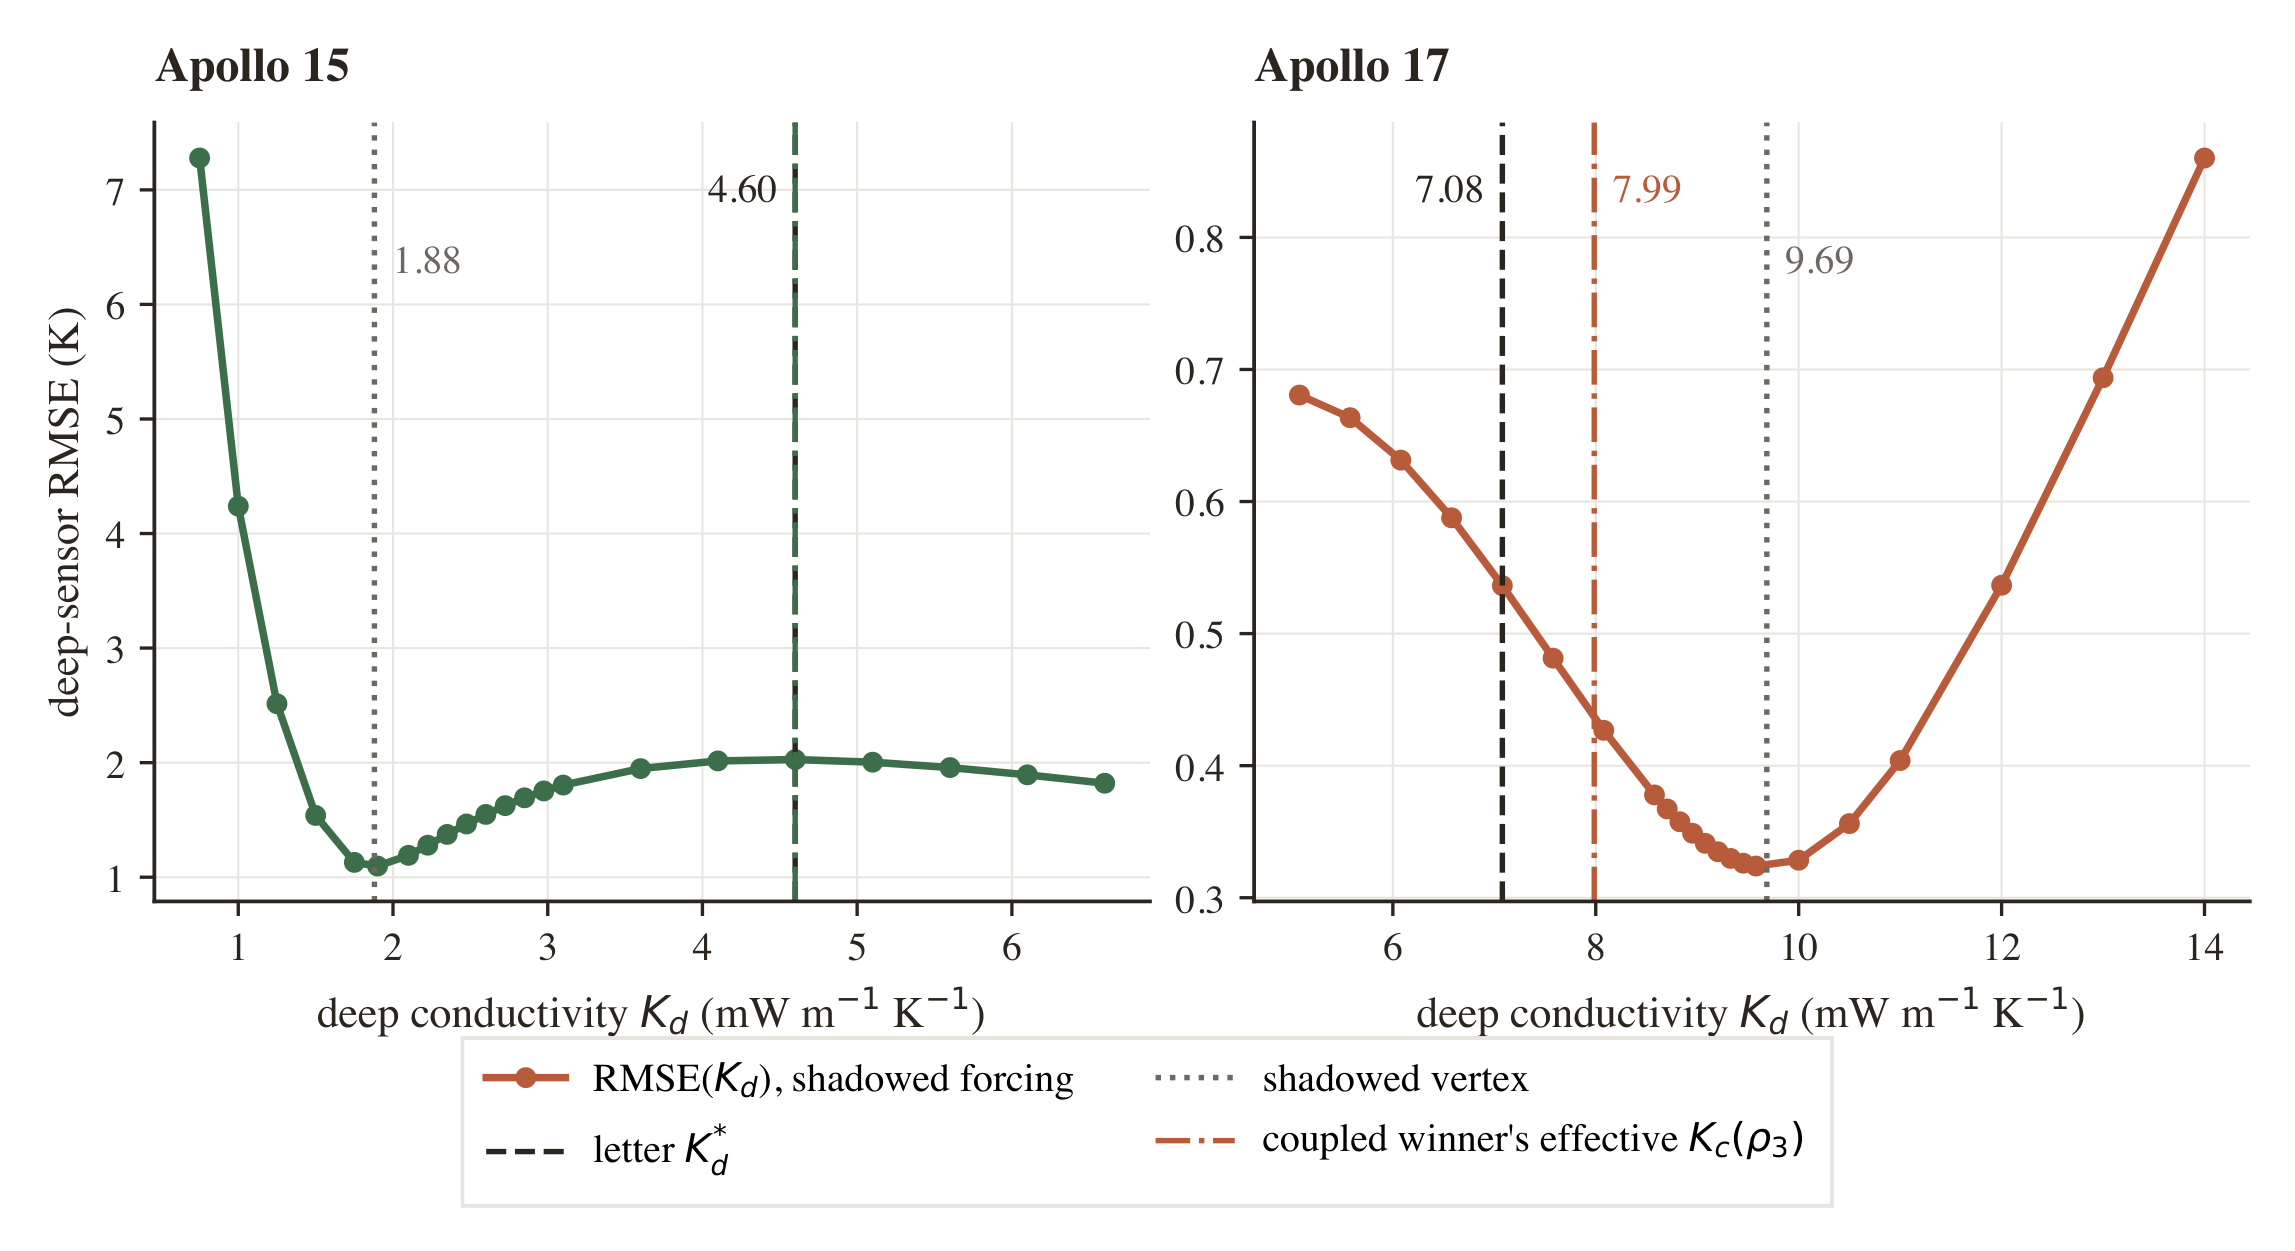
\includegraphics[width=0.86\linewidth]{explainer_kd_bowl.pdf}
  \caption{The retrieval bowl under shadowed forcing (zero new solves; from the
  extended $K_d$ sweep). Dashed = letter $K_d^{*}$; dotted = shadowed-forcing
  vertex; dash-dot = the coupled winner's effective deep conductivity. At A15
  the dashed and dash-dot lines coincide because its winner's deep density
  equals Hayne's; at A17 the winner sits above $K_d^{*}$ --- the degeneracy,
  drawn.}
\end{figure}

% ── 6 tiers ──────────────────────────────────────────────────────────────────
\shead{6.\ \ So how should $K_d$ be found?}
Because of the degeneracy, don't fit both freely. Three tiers:

\begin{figure}[h]\centering
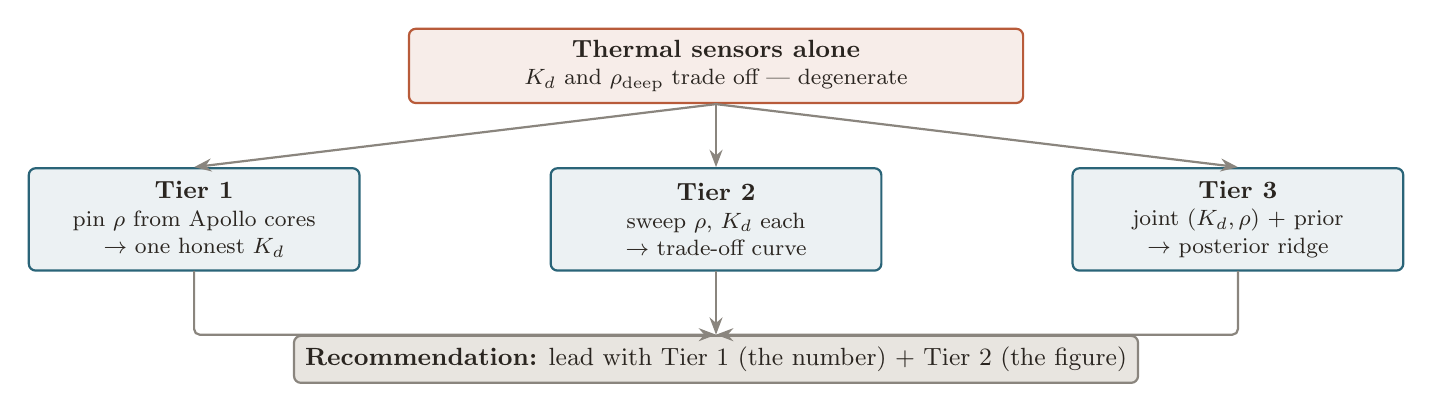
\begin{tikzpicture}
  \node[warnbox, minimum width=78mm] (prob)
    {\textbf{Thermal sensors alone}\\[-1pt]
     {\footnotesize $K_d$ and $\rho_\mathrm{deep}$ trade off --- degenerate}};
  \node[newbox, below left=8mm and 6mm of prob, minimum width=42mm,
        minimum height=13mm] (t1)
    {\textbf{Tier 1}\\[-1pt]{\footnotesize pin $\rho$ from Apollo cores}\\[-1pt]
     {\footnotesize $\to$ one honest $K_d$}};
  \node[newbox, below=8mm of prob, minimum width=42mm, minimum height=13mm] (t2)
    {\textbf{Tier 2}\\[-1pt]{\footnotesize sweep $\rho$, $K_d$ each}\\[-1pt]
     {\footnotesize $\to$ trade-off curve}};
  \node[newbox, below right=8mm and 6mm of prob, minimum width=42mm,
        minimum height=13mm] (t3)
    {\textbf{Tier 3}\\[-1pt]{\footnotesize joint $(K_d,\rho)$ + prior}\\[-1pt]
     {\footnotesize $\to$ posterior ridge}};
  \node[greybox, below=8mm of t2, minimum width=96mm] (rec)
    {\textbf{Recommendation:} lead with Tier 1 (the number) $+$ Tier 2 (the figure)};
  \draw[arr] (prob.south) -- (t1.north);
  \draw[arr] (prob.south) -- (t2.north);
  \draw[arr] (prob.south) -- (t3.north);
  \draw[arr] (t1.south) |- (rec.north);
  \draw[arr] (t2.south) -- (rec.north);
  \draw[arr] (t3.south) |- (rec.north);
\end{tikzpicture}
\caption{Anchor hierarchy: site $K_d^{*}$ = anchor $\cdot$ Hayne global 3.4 =
named baseline $\cdot$ shadowed vertices (1.88 / 9.69) = diagnostic only.}
\end{figure}

% ── 7 results ────────────────────────────────────────────────────────────────
\shead{7.\ \ The results}
\begin{table}[h]\centering\small
\begin{tabular}{lcc}
\toprule
model (shadowed forcing) & A15 RMSE (K) & A17 RMSE (K)\\
\midrule
homogeneous (constant $K$, constant $\rho$) & 2.31 & 3.76\\
Hayne \textbf{global} $K_d=3.4$             & 1.90 & 0.71\\
Hayne continuous at site $K_d^{*}$          & \rmsehayAfif & \rmsehayAsev\\
best \textbf{cp} (density $\to$ heat capacity) & \rmsecpAfif & \rmsecpAsev\\
best \textbf{coupled} (density $\to$ conductivity) & \textbf{\rmsecKAfif} & \textbf{\rmsecKAsev}\\
\bottomrule
\end{tabular}
\caption{Layering wins: the coupled model beats homogeneous by ${\sim}2.6\times$
(A15) and ${\sim}10\times$ (A17). Heat capacity alone barely moves the fit
($\le0.7$ K); density-through-conductivity spans ${\sim}4$ K.}
\end{table}

\begin{figure}[h]\centering
  \includegraphics[width=0.72\linewidth]{poster_profiles.pdf}
  \caption{Validation against the Apollo HFE deep sensors (circles). The
  density-coupled line (RMSE 0.90 / 0.36 K) threads the measurements where the
  smooth models miss.}
\end{figure}

\begin{figure}[h]\centering
  \includegraphics[width=0.74\linewidth]{poster_sens.pdf}
  \caption{Sensitivity. \emph{Top:} RMSE spread of all 162 configs --- cp tight,
  coupled wide. \emph{Bottom:} RMSE over the layer-boundary plane (green =
  good); the mid$|$deep break wants to sit high ($z_2=30$ cm) at both sites.}
\end{figure}

\noindent\textbf{Robustness \& geology.} A free bootstrap over the stored
temperatures shows the \emph{improvement} is solid (coupled best-RMSE 95\% CIs
0.85\,[0.26,1.08] / 0.35\,[0.25,0.43] K) though the exact A15 triple is
degenerate --- the robust claim is the \emph{class} of profile. And the deep
densities retrieved \emph{thermally} (1800 / 1900) match those Apollo measured
\emph{mechanically} (1825 / 1960 kg\,m$^{-3}$; Grott et al.), ordering included.

% ── 8 caveats ────────────────────────────────────────────────────────────────
\shead{8.\ \ Honest caveats (know these cold)}
\begin{itemize}
  \item \textbf{Topography enters twice, with opposite signs.} The shadowing
    itself cools the deep sensors by \shadowcoolAfif/\shadowcoolAsev\,K
    (A15/A17); the same terrain glows in the IR and reflects sunlight, warming
    them by $+\svfdtirAfif$/$+\svfdtirAsev$\,K. So cooling dominates at A15, but
    the warming \emph{wins} at A17. Two opposing first-order channels from the
    same DEM horizons; the terrain-radiation channel is a diagnostic, not yet
    folded into the fits --- a full re-sweep with it on is the next step.
  \item \textbf{$K_d$--density degeneracy} (\S5) --- the central limitation; a
    joint $(K_d,\rho)$ retrieval with a core-density prior resolves it.
  \item \textbf{16 ppd DEM} (${\sim}1.9$ km/px) under-resolves A17's near
    massifs, so its horizons are a \emph{lower} bound; solar declination is
    fixed at $0^\circ$; $\chi$ and $Q_b$ are held at the letter's values (they
    dominate its error budget).
\end{itemize}

% ── 9 question bank ──────────────────────────────────────────────────────────
\newcommand{\qa}[2]{\smallskip\par\noindent{\color{teal}\textbf{Q.\ #1}}\\*
  \noindent#2\par}

\shead{9.\ \ If someone asks you\,\dots\ (a question bank)}
Every answer below is short on purpose --- say the first sentence, and only go
deeper if they push. The numbers are all in \S11.

\smallskip\noindent{\bfseries\color{dim} METHOD \& SOLVER}
\qa{Why not just fit $K_d$ and the deep density together?}{Because they are
\emph{degenerate} (\S5). The deep temperature gradient is essentially
$Q_b/K_\mathrm{deep}$, and both a higher $K_d$ \emph{and} a denser deep layer
raise $K_\mathrm{deep}$ --- the sensors see only the product. We hold $K$ at the
letter's certified $K_d^{*}$ and vary density (or the reverse), and report the
result as \emph{one} deep-gradient constraint, not two independent numbers.}
\qa{What is the ``flux-anchored solver,'' and why is it ${\sim}20\times$
faster?}{Brute force time-steps thousands of lunations until the column stops
drifting. Instead we \emph{anchor} the mean profile below the rectification zone
($z_0=55$ cm), where the diurnal wave is dead and $d\langle
T\rangle/dz=(Q_b-u_\mathrm{rect})/K$, then reconstruct the deep column from that
closure. About 0.6\,s per solve versus ${\sim}26$ min, verified identical to
$<1$\,mK.}
\qa{How do you know a solve actually converged?}{Convergence is
\emph{anchor-temperature stability} (drift $<5$\,mK between cycles), not a fixed
cycle count. The winning configurations, re-run at the production spin-up
($n{=}96$), agree to $\leq\driftmax$\,mK.}
\qa{What's the difference between the \emph{cp} and \emph{coupled} branches?}{In
\emph{cp}, density enters only the heat capacity $\rho c_p$; $K$ stays at the
site $K_d^{*}$. In \emph{coupled}, density \emph{also} sets the contact
conductivity through the Hayne form's own linear $K_c(\rho)$ --- no new
constants. cp can only shift the whole profile; coupled can \emph{tilt} the deep
gradient onto the sensors, which is why it wins.}

\smallskip\noindent{\bfseries\color{dim} DATA}
\qa{Which sensors, and why exclude some?}{The HFE deep sensors, below 80\,cm.
Above that the fibreglass borestem conducts the surface wave downward and biases
the equilibrium temperature. Each sensor gives one equilibrium temperature from
a quiet late-mission window of the restored 1971--77 record.}
\qa{Is the probe metal --- doesn't it short the heat?}{No --- it is a
fibreglass/epoxy borestem, deliberately low-conductivity. The shallow-sensor
exclusion above already guards against the residual down-conduction.}

\smallskip\noindent{\bfseries\color{dim} SHADOWING \& TERRAIN}
\qa{How much does shadowing actually matter?}{It removes \lossAfif/\lossAsev\%
of the insolation \emph{energy}, which cools the deep sensors by
\shadowcoolAfif/\shadowcoolAsev\,K. But the terrain that blocks the Sun also
radiates back ($+\svfdtirAfif/+\svfdtirAsev$\,K), so the net is sub-K --- and at
A17 the warming actually wins.}
\qa{Isn't a 16 ppd DEM too coarse, especially for A17?}{Honestly, yes for the
near-field massifs --- so A17's horizons (and its shadowing) are a
\emph{lower} bound. A15's Apennine front is a broad feature that \emph{is}
resolved. Better topography would only strengthen the shadowing case, not weaken
it.}
\qa{Why fix the solar declination at $0^\circ$?}{It's second-order for a
monthly-averaged profile; the $\pm1.5^\circ$ seasonal wobble is a refinement,
not a driver of these results.}

\smallskip\noindent{\bfseries\color{dim} RESULTS \& SIGNIFICANCE}
\qa{How do you rule out curve-fitting?}{The cross-site test: move each site's
best structure to the \emph{other} site. It degrades gracefully but still beats
homogeneous ($\xferatAfif$\,K at A15, $\xferatAsev$\,K at A17). Curve-fit
parameters would not transfer; physical ones do.}
\qa{How robust is the winning density triple?}{The \emph{improvement} over
homogeneous is bootstrap-solid (coupled best-RMSE 95\% CI \bootcicKAfif\ /
\bootcicKAsev\,K, far under the homogeneous baselines). The exact A15 triple is
\emph{not} robust (\stabcKAfif\% bootstrap stability) --- so we claim the
\emph{class} of profile (denser-than-Hayne surface, shallow compaction step),
never one specific triple.}
\qa{Do the retrieved densities mean anything physically?}{Yes --- the deep
densities retrieved \emph{thermally} (1800 / 1900) match those Apollo measured
\emph{mechanically} in the drive cores (1825 / 1960 kg\,m$^{-3}$; Grott et al.),
ordering included. Independent confirmation, not an input.}
\qa{So is the deep conductivity 4.6 or 7.1?}{Those are the letter's per-site
$K_d^{*}$ under Hayne density. Deep conductivity and deep density are two views
of the \emph{same} deep-gradient constraint --- we report one number, not two
independent retrievals.}

\smallskip\noindent{\bfseries\color{dim} IF THEY PROBE A WEAK SPOT}
\qa{Your shadowed re-retrieval gives $K_d=1.88$ mW at A15 --- that's a huge
drop!}{Don't lead with that number. That vertex is a \emph{diagnostic} from a
coarse, mixed-resolution re-sweep sitting near the physical conductivity floor;
it is not a headline retrieval. The robust result is the density story and the
${\sim}2.6\times$/$10\times$ improvement over homogeneous.}
\qa{Isn't holding $\chi$ and $Q_b$ fixed a problem?}{They are the letter's
certified values and dominate \emph{its} error budget; varying them is the
letter's job. Fixing them here is what lets us isolate the density and
topography effects cleanly.}

% ── 10 walkthrough ───────────────────────────────────────────────────────────
\shead{10.\ \ The 60-second walkthrough (what to say, pointing where)}
\begin{enumerate}[leftmargin=1.6em, itemsep=1.5pt]
  \item \textbf{Sites:} ``Two places on the Moon have subsurface temperature
    ground truth --- the Apollo 15 and 17 heat-flow boreholes.''
  \item \textbf{Model schematic:} ``We reuse one certified thermal solver and
    add two things: the real terrain's shadow from the DEM, and a 3-layer
    density column instead of one smooth curve.''
  \item \textbf{Pipeline:} ``Every candidate column runs through the same
    pipeline --- 650 solves.''
  \item \textbf{Profiles + table:} ``The layered, density-coupled model lands on
    the sensors where the smooth homogeneous model misses by 2--4 kelvin.''
  \item \textbf{Sensitivity box plots:} ``The lever is conductivity, reached
    \emph{through} density --- heat capacity alone can't do it.''
  \item \textbf{Transfer matrix:} ``And swap the two sites' structures --- it
    degrades gracefully but still beats homogeneous. That's physics, not
    curve-fitting.'' \emph{Then stop and invite questions.}
\end{enumerate}

% ── 11 numbers card ──────────────────────────────────────────────────────────
\shead{11.\ \ Numbers at your fingertips}
\begin{table}[H]\centering\small
\setlength{\tabcolsep}{5pt}\renewcommand{\arraystretch}{1.15}
\begin{tabular}{lcc}
\toprule
 & \textbf{Apollo 15} & \textbf{Apollo 17}\\
\midrule
Location (lat, lon) & 26.1$^\circ$N, 3.6$^\circ$E & 20.2$^\circ$N, 30.8$^\circ$E\\
Horizon max / insolation loss & \horAfif$^\circ$ / \lossAfif\% & \horAsev$^\circ$ / \lossAsev\%\\
Sky-view factor & \svfAfif & \svfAsev\\
Shadow cooling at sensors & \shadowcoolAfif\,K & \shadowcoolAsev\,K\\
Terrain-IR warming & $+\svfdtirAfif$\,K & $+\svfdtirAsev$\,K\\
Certified $K_d^{*}$ (letter) & \kdstarAfif & \kdstarAsev\ mW\,m$^{-1}$K$^{-1}$\\
Best coupled RMSE & \textbf{\rmsecKAfif}\,K & \textbf{\rmsecKAsev}\,K\\
Homogeneous RMSE & \rmsehomAfif\,K & \rmsehomAsev\,K\\
Improvement over homogeneous & ${\sim}2.6\times$ & ${\sim}10\times$\\
Cross-site (structure moved) & \xferatAfif\,K & \xferatAsev\,K\\
Deep density: thermal / core & 1800 / 1825 & 1900 / 1960 kg\,m$^{-3}$\\
\bottomrule
\end{tabular}
\caption{Everything you might be asked for, one glance. Shared constants:
$K_s=7.4\times10^{-4}$, $H=6$ cm, $\chi=2.7$, $Q_b=21/16$ mW\,m$^{-2}$, anchor
$z_0=55$ cm; 650 configurations; ${\sim}0.6$ s/solve.}
\end{table}

\shead{12.\ \ One-sentence takeaway}
Using the letter's certified engine, real terrain shadowing plus a 3-layer
density column reproduces the Apollo borehole temperatures far better than any
smooth homogeneous model, and the densities it retrieves \emph{thermally} match
those Apollo measured \emph{mechanically} --- with the honest caveat that deep
conductivity and deep density are two views of the same quantity.

\end{document}
